{\let\clearpage\relax \chapter{Funkcjonalność}}
Nasz projekt będzie oferował użytkownikom następujące funckjonalności:

\section{Interfejs graficzny}

Użytkownikowi zostanie udostępniony interfejs graficzny z poziomu przeglądarki internetowej. Za jego pomocą będzie odbywać się wszelka interakcja użytkownika z grą, a będzie się ona składać z następujących etapów:

\
\begin{enumerate}
	\item Wprowadzenie wojownika poprzez wpisanie w odpowiednim polu kodu lub wczytanie istniejącego już zestawu instrukcji z pliku lub bazy danych (opcjonalnie, patrz \ref{instrukcje});

	\item Obserwacja walki wraz z możliwością ingerencji w ustawienia, m. in. szybkości rozgrywki;

	\item Wyświetlenie interesujących danych dotyczących walki;

	\item Zapis wojownika/statystyk do pliku lub bazy danych (opcjonalnie, patrz \ref{instrukcje}).
	
\end{enumerate}

\

Zamierzamy zwizualizować stan rywalizacji jako dwuwymiarową tablicę, jak na rys. \ref{gametable}, gdzie każdej komórka odpowiadać będzie adresowi w pamięci. Kolory poszczególnych komórek odpowiadać będą procesom użytkowników, co umożliwi ocenę, jaką część pamięci kontroluje każdy z graczy.

\

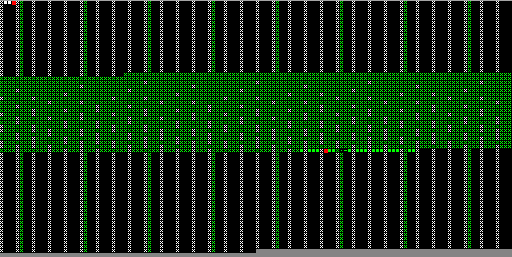
\includegraphics[width=\linewidth]{utils/pic1.png}
\captionof{figure}{Przykładowa plansza obrazująca stan rozgrywki}
\label{gametable}

\

\section{Tworzenie wojowników (Wprowadzanie instrukcji)}
Każdy wojownik (program w języku RedCode) będzie się składał zestawu instrukcji, opisanych w punkcie \ref{instrukcje}. Gracze będą mieli możliwość wprowadzenia tych instrukcji do programu na kilka sposobów:

\
\begin{enumerate}
	\item Wprowadzenie instrukcji z poziomu interfesju graficznego lub z pliku tekstowego:
	\newline
		Gracz dostanie możliwość tworzenia programu poprzez wpisanie kodu w wyznaczonym miejscu interfejsu graficznego, lub załadowania kodu z pliku tekstowego. Zostanie zaimplementowana walidacja kodu pod względem poprawności składni i informacją zwrotną dla użytkownika.
	
	\item Pobranie kodu z relacyjnej bazy danych, np. SQLite (opcjonalnie, patrz \ref{instrukcje}).
\end{enumerate}

\section{Instrukcje RedCode}
Językiem, w którym gracze będą pisali swoje programy, będzie Redcode. Zestaw instrukcji, które zamierzamy zaimplementować, jest zgodny ze standardem \textit{ICWS '88} i zawiera polecenia: \textit{MOV, ADD, SUB, JMP, JMZ, JMN, CMP, SLT, DJN, SPL, NOP}.
\label{instrukcje}

\section{Integracja z bazą danych (funkcjonalność dodatkowa)}

Zaimplementowanie powyższych funkjonalności jest naszym priorytetem. Integracja z bazą danych jest elementem, który zostanie dodany, jeśli pozostałe etapy zostaną ukończone pomyślnie przed terminem oddania projektu. Planujemy połączenie z bazą relacyjną, np SQLite. Umożliwi to zapis i odczyt wcześniej utworzonych zawodników i statystyk ich dotyczących.

\label{database}
